\section{Results and Discussion}
\label{sec:results}

This section presents computational results for three scenarios (16, 36, and 64 turbines), analyzing quantitative metrics, qualitative layouts, and comparisons with state-of-the-art methods.

\subsection{Quantitative Performance Analysis}

\subsubsection{Pareto Front Characteristics}

Table \ref{tab:pareto_summary} summarizes the Pareto fronts for each scenario. The framework identified 29, 4, and 5 unique non-dominated solutions for the 16, 36, and 64-turbine cases, respectively. The 16-turbine case exhibits the richest trade-off space, likely due to co-optimization of multiple decision variables. This compares favorably with recent NSGA-II studies: Zheng et al. \cite{Zheng2025NSGA2} reported 13 Pareto solutions, while Konatham et al. \cite{Konatham2024NSGA2} identified 4 solutions.

\begin{table}[ht]
\caption{Summary of Pareto front characteristics for the three test scenarios.}
\label{tab:pareto_summary}
\centering
\begin{tabular}{@{}lcccc@{}}
\toprule
\textbf{Scenario} & \textbf{Unique Solutions} & \textbf{Max AEP (GWh)} & \textbf{Min Cost (M USD)} & \textbf{Max Cost (M USD)} \\
\midrule
16 turbines & 29 & 461.76 & 0.38 & 0.77 \\
36 turbines & 4 & 939.59 & 1.57 & 1.77 \\
64 turbines & 5 & 1,432.29 & 3.16 & 3.39 \\
\bottomrule
\end{tabular}
\end{table}

The Pareto fronts exhibit clear trade-offs: the 16-turbine case spans 445.53--461.76 GWh (3.5\% variation) with costs ranging from 0.38--0.77 M USD (101.4\% variation). For larger scales, cost variations decrease (13.0\% for 36 turbines, 7.5\% for 64 turbines), suggesting more efficient cost-energy balancing. As noted by Wang et al. \cite{Wang2019Integrated}, the match between topology and cable sizing drives economy. Our 64-turbine results prioritize 240\,mm$^2$ cables while maintaining uniform section strategy \cite{Jiang2025Review, Alencar2026Flexible}.

\subsubsection{Evolution of the Optimization Process}

Figure \ref{fig:metrics_evolution} shows the evolutionary dynamics for the 16-turbine scenario. Phase 1 (Generations 0--471) reaches a gross AEP plateau at 466.71 GWh. Phase 2 introduces infrastructure variables and NSGA-II, reducing cabling cost from ~850 kUSD to 380--480 kUSD (45--56\% reduction) while Net AEP stabilizes at 455--458 GWh. This confirms that integrated planning outperforms separate optimization, as demonstrated by Jin et al. \cite{Jin2019PowerLoss} (3.14\% cost reduction) and Tao et al. \cite{Tao2025TwoStage} (4.72\% AEP increase). Our Smart Seeding strategy bridges exploration and exploitation phases \cite{Silva2025Layout}.

\begin{figure*}[ht]
\centering

\includegraphics[width=0.95\textwidth]{TESTE/TESTE_16_PARA_ARTIGO/metrics_evolution.png}
\caption{Evolution of AEP and cabling cost across generations (16 turbines). Phase 1 (blue) maximizes gross AEP; Phase 2 (green) balances Net AEP and cost using NSGA-II.}
\label{fig:metrics_evolution}
\end{figure*}

\subsection{Qualitative Layout Analysis}

\subsubsection{Comparative Solutions Across Scenarios}

Figure \ref{fig:comparative_layouts_all} presents three archetypal solutions per scenario. For 16 turbines, minimum cost and knee point are identical (445.53 GWh, \$380k), using 70 mm² cables (30.26 km). Maximum AEP (461.76 GWh, \$766k) requires 95 mm² cables (44.90 km), representing a 101.6\% cost increase for 3.5\% AEP gain. For 36 turbines, cable cross-section (150 vs. 185 mm²) drives cost more than length, aligning with Shen et al. \cite{Shen2023Ring} (4--8\% cost reductions). The 64-turbine case shows balanced trade-offs: 9.6\% AEP increase requires 9.6\% cost premium, with all solutions using 240 mm² cables.

\begin{figure*}[ht]
\centering
\begin{subfigure}[b]{\textwidth}
\centering

\includegraphics[width=0.95\textwidth]{TESTE/TESTE_16_PARA_ARTIGO/comparative_layouts_1x3.png}
\caption{16 turbines: Min Cost/Knee (AEP: 445.53 GWh, Cost: \$380k), Max AEP (AEP: 461.76 GWh, Cost: \$766k)}
\label{fig:comparative_16}
\end{subfigure}
\\[0.5cm]
\begin{subfigure}[b]{\textwidth}
\centering
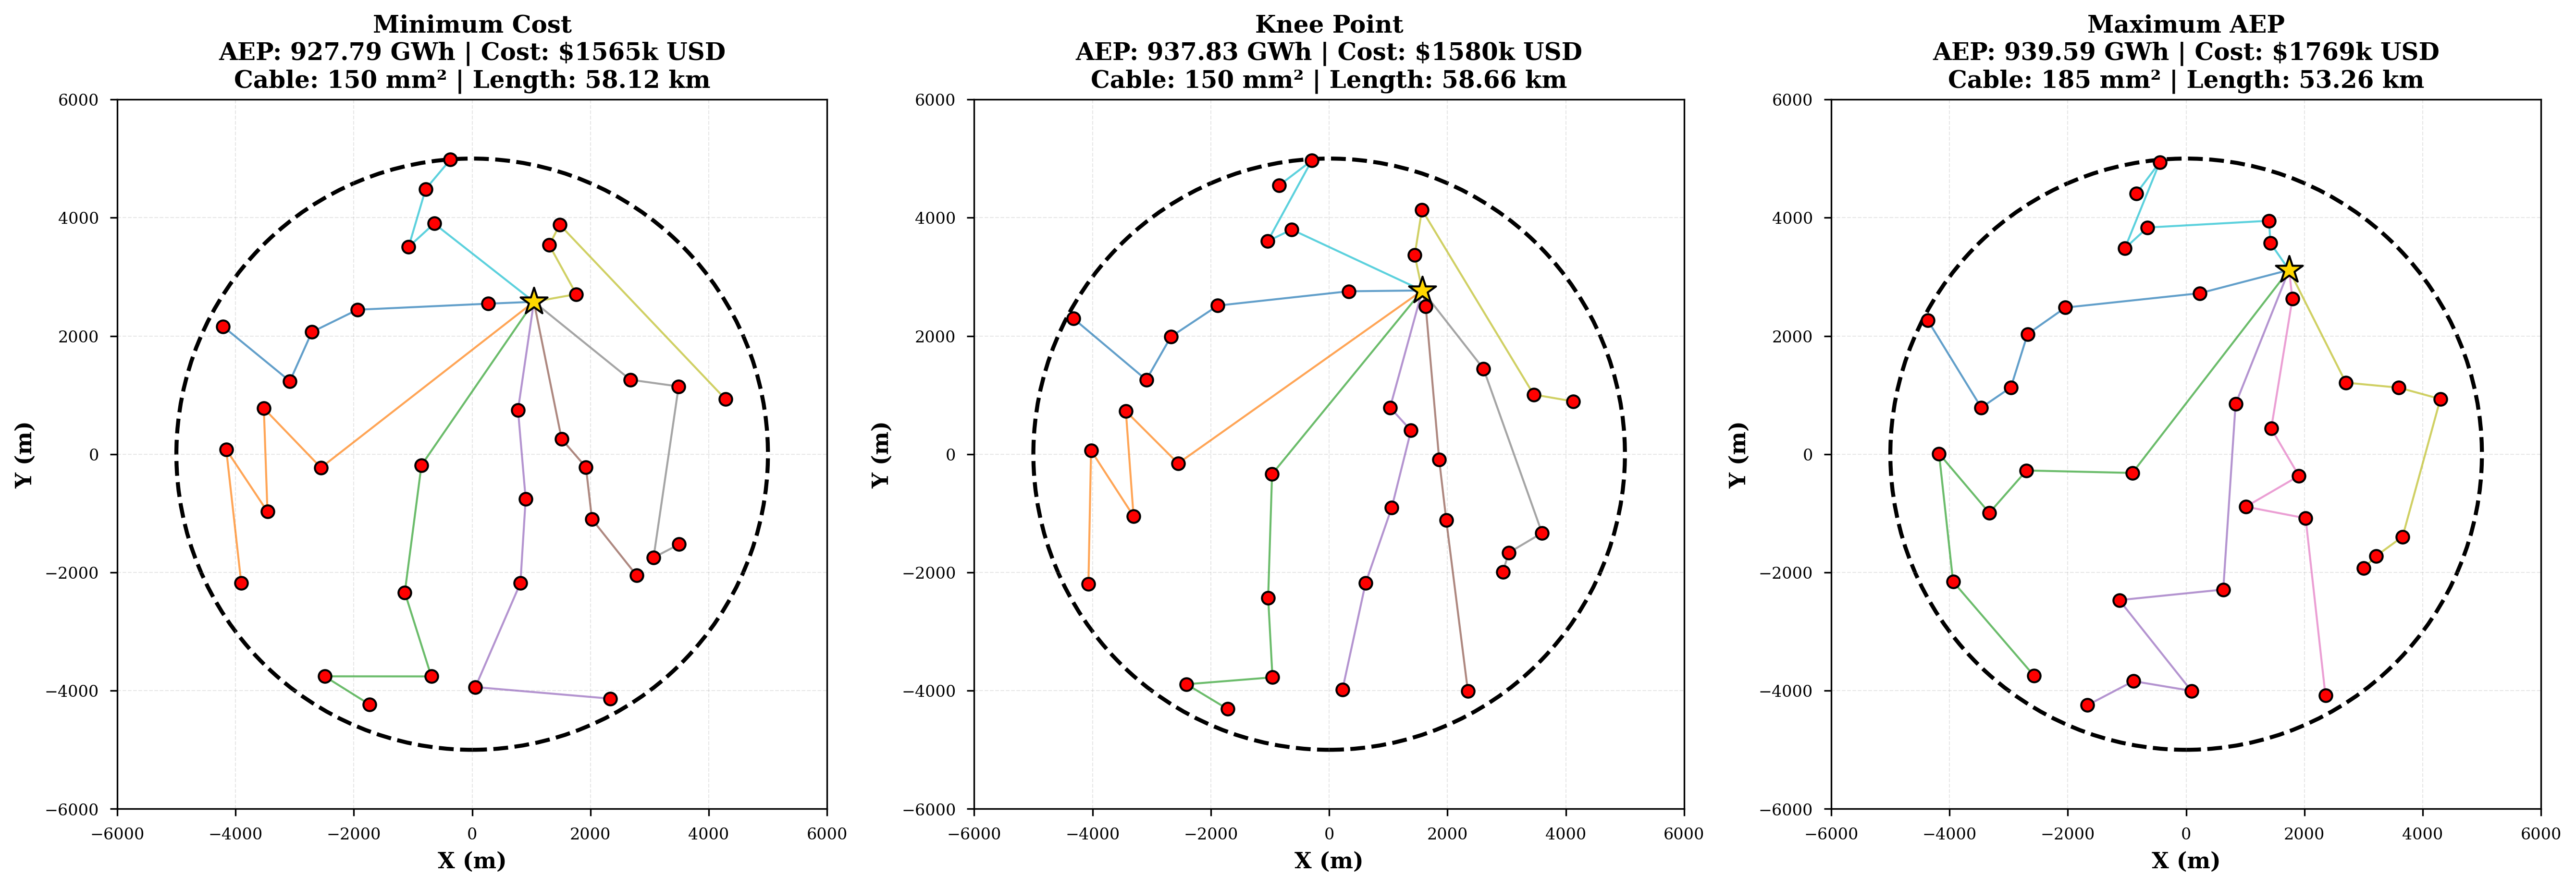
\includegraphics[width=0.95\textwidth]{TESTE/TESTE_36_PARA_ARTIGO/comparative_layouts_1x3.png}
\caption{36 turbines: Min Cost (AEP: 927.79 GWh, Cost: \$1,565k), Knee (AEP: 937.83 GWh, Cost: \$1,580k), Max AEP (AEP: 939.59 GWh, Cost: \$1,769k)}
\label{fig:comparative_36}
\end{subfigure}
\\[0.5cm]
\begin{subfigure}[b]{\textwidth}
\centering
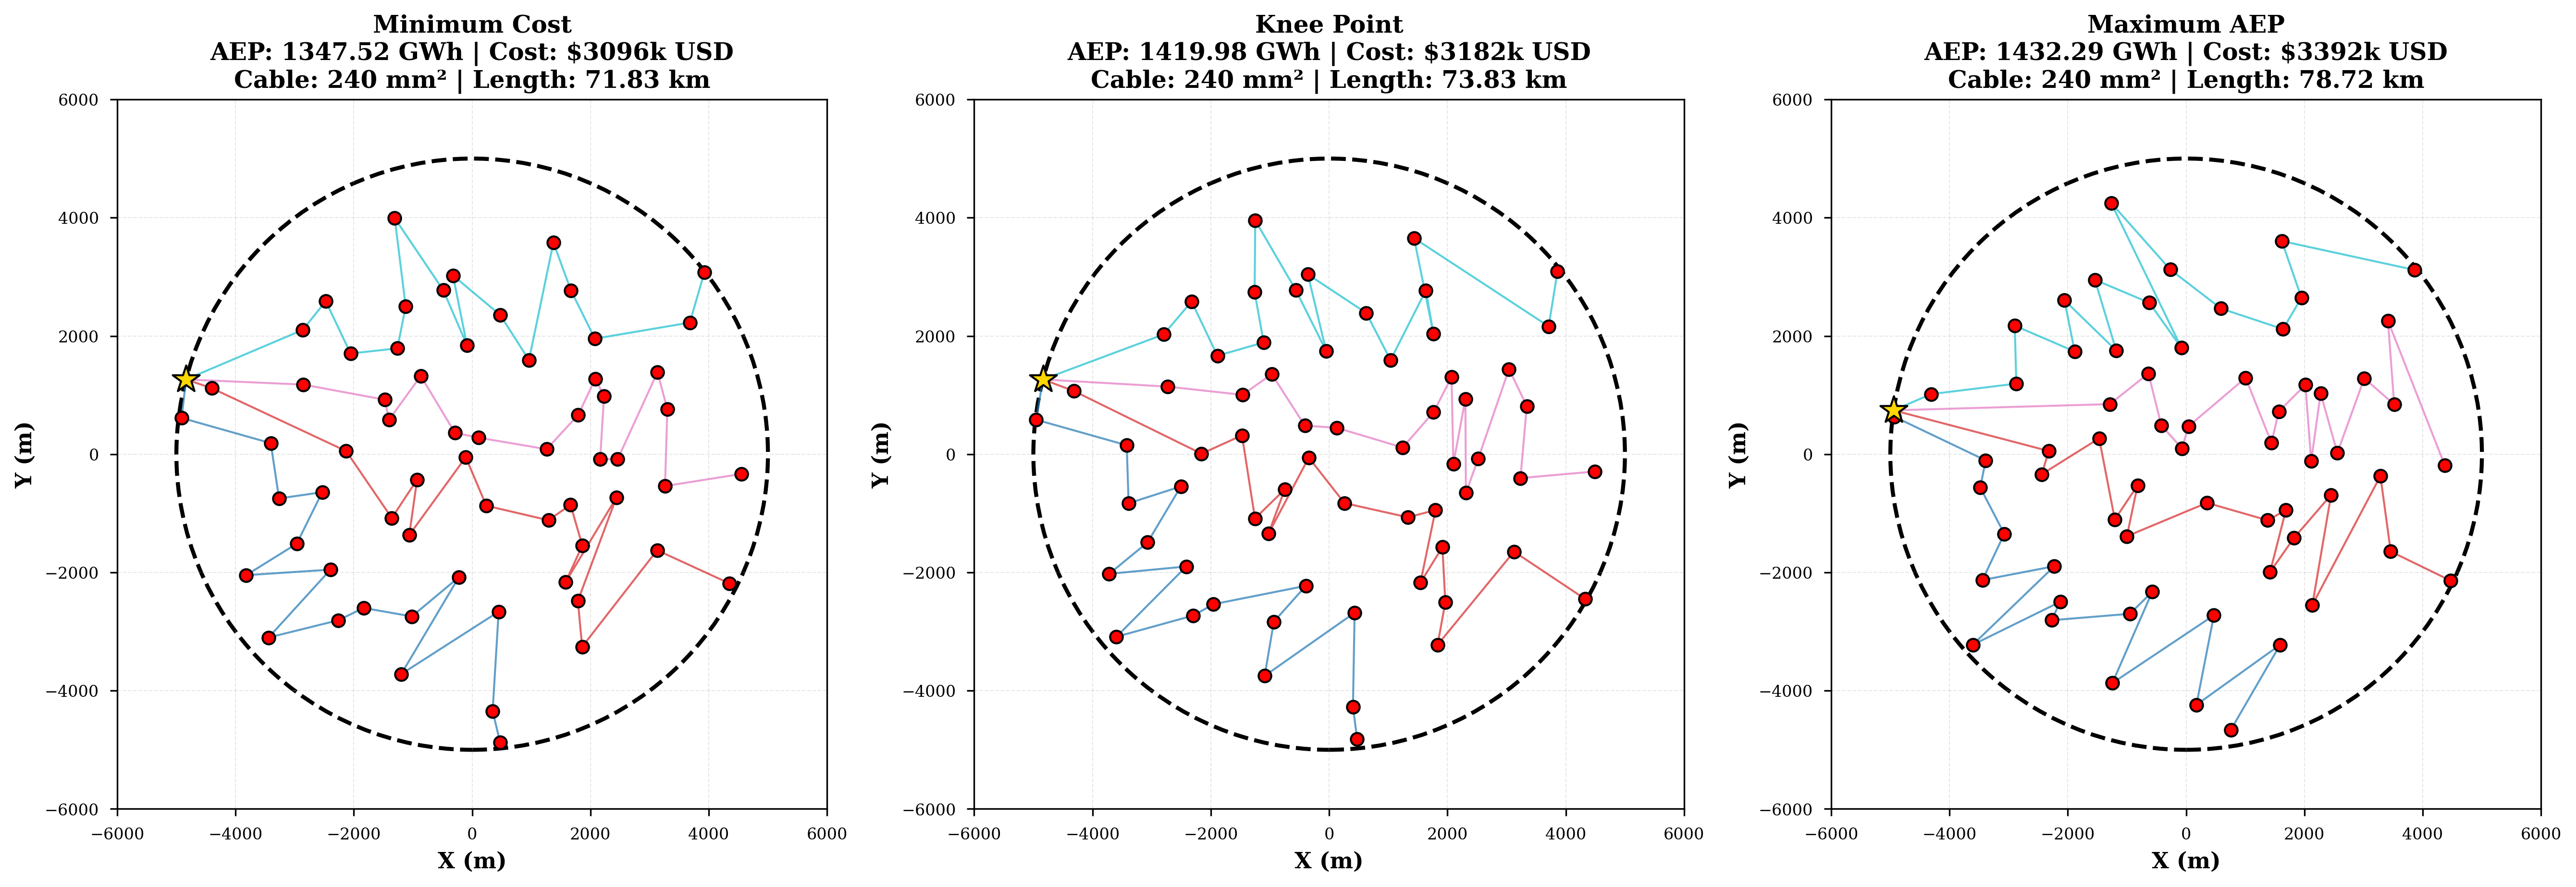
\includegraphics[width=0.95\textwidth]{TESTE/TESTE_64_PARA_ARTIGO/comparative_layouts_1x3.png}
\caption{64 turbines: Min Cost (AEP: 1,347.52 GWh, Cost: \$3,096k), Knee (AEP: 1,419.98 GWh, Cost: \$3,182k), Max AEP (AEP: 1,432.29 GWh, Cost: \$3,392k)}
\label{fig:comparative_64}
\end{subfigure}
\caption{Comparative layouts showing Min Cost, Knee Point, and Max AEP solutions. Colors represent cable strings, demonstrating non-crossing topology guaranteed by angular sector partitioning.}
\label{fig:comparative_layouts_all}
\end{figure*}

The angular sector grouping ensures planar cable graphs without geometric repair heuristics, as required in \cite{Alencar2026Flexible, Ye2023Path}. This achieves the 60-fold computational reduction suggested by Alencar et al. \cite{Alencar2026Flexible} while maintaining full turbine mobility, often restricted in high-dimensional solvers \cite{Fischetti2015MILP, Machado2024Hybrid}.

\subsubsection{Hierarchical Strategy Impact}

Figure \ref{fig:phase1_vs_phase2} illustrates the hierarchical strategy. Phase 1 increases gross AEP from 366.56 to 466.71 GWh (27.3\%). Phase 2 refines this layout, achieving 445.53 GWh Net AEP (4.5\% below Phase 1 gross) at \$380k, effectively bridging energy optimization and economic feasibility. This two-phase decomposition addresses the co-optimization challenge by first exploring the $2n$-dimensional layout space, then refining in the full $(2n+3)$-dimensional space, reducing convergence risk to poor local optima.

\begin{figure*}[ht]
\centering

\includegraphics[width=0.95\textwidth]{TESTE/TESTE_16_PARA_ARTIGO/phase1_vs_phase2_comparison.png}
\caption{Hierarchical optimization: (a) Phase 1 Initial (AEP: 366.56 GWh), (b) Phase 1 Best (AEP: 466.71 GWh), (c) Phase 2 Knee Point (AEP: 445.53 GWh, Cost: \$380k).}
\label{fig:phase1_vs_phase2}
\end{figure*}

\subsection{Co-Optimization Benefits and Comparison with Literature}

Unlike methods that fix turbine positions \cite{Alencar2026Flexible, Machado2024Hybrid} or optimize separately \cite{Tao2025TwoStage}, our framework co-optimizes layout, substation location, and cable topology. Mobile substation optimization, evident in Fig. \ref{fig:comparative_layouts_all}, enables simultaneous minimization of cable lengths and Joule losses, as emphasized by Moon et al. \cite{Moon2015Optimal}.

Electrical losses account for ~4.5\% of gross AEP in the 64-turbine case, directly impacting LCOE. Jin et al. \cite{Jin2019PowerLoss} showed that power loss models reduce total costs by 3.14\%. Our framework extends this by co-optimizing all variables, allowing informed trade-offs between wake losses and electrical losses.

Quantitatively, our results compare favorably: Yuan and Tang \cite{Yuan2025ACO} reported 3.82\% cost reductions, He et al. \cite{He2025Topology} achieved 7.27\%, while our framework provides complete Pareto fronts (29 solutions for 16 turbines) rather than single optima. The hierarchical strategy enables efficient exploration of high-dimensional spaces (up to 131 variables for 64 turbines), addressing the co-optimization challenge that limits scalability in existing methods \cite{Machado2024Hybrid}.
